\section{\textit{Stress test} рада сервера}

До сада, фокус је био на имплементацији сервера, али ни у једном тренутку није извршена провера да ли обе имплементације функционишу како је специфицирано и да ли у неким случајевима улазе у недефинисана стања и доводе до пада сервера. У оквиру овог поглавља биће описан начин на који је извршена верификација правилног рада обе имплементације.\\

За потребе тестирања коришћен је алат \textit{Apache JMeter} \cite{jmeter}који омогућава дефинисање тест сценариа за тестирање сервера, који може да обухвати велики број паралелних захтева ка серверу, као и да омогући накнадну анализу извршеног сценариа.\\

За потребе тестирања тренутних имплементација дефинисан је сценарио од:
\begin{itemize}
    \item 10000 паралелних \textit{GET}  захтева, где сваки захтев чита различит елемент мапе.
    \item 10000 паралелних \textit{PUT}  захтева, где сваки захтев уписује елемент мапе који до тада није постојао у мапи.
    \item 20000 паралелних \textit{PUT}  захтева, где свака два захтева покушавају да измене исти елемент који већ постоји у мапи.
\end{itemize}
Овим сценариом успевамо да тестирамо све случајеве конкурентног приступа наведених у поглављу \ref{list:concurrent_cases}. Конкретан фајл са конфигурацијом сценариа може се наћи на путањи \url{https://github.com/stojanovic00/rust-go-server-comp/blob/main/profiling/stress_testing/rust_testing.jmx}. Подаци који су се користили за тестирање генерисани су наменском \textit{Go} скриптом \verb|test_data_generator| која генерише насумичне вредности за \textit{descritpion}  и  \textit{value} поља ентитета за задати број ентитета, док поља \textit{id} инкрементира за један почевши од нуле. Код \verb|test_data_generator| скрипте може се наћи на путањи \url{https://github.com/stojanovic00/rust-go-server-comp/tree/main/profiling/stress_testing/test_data_generator}\\

Табеле са резултатима приказане на сликама \ref{fig:stress_rust} и \ref{fig:stress_go} јасно приказују да је свих 40000 захтева упућених ка оба сервера обрађено са 0\% грешака (колона \textit{Error \%}). Остале метрике приказане у табели нису толико меродавне због тога што је \textit{Apache JMeter} намењен за тестирање у окружењу где постоји тест сервер и сервер на коме се покреће \textit{Apache JMeter}, док је за потребе овог тестирања \textit{Apache JMeter} покретан на истом серверу на којем се налазе и имплементације сервера, али за потребе верификације исправног рада имплементација сервера покретање \textit{Apache JMeter} у оваквом окружењу је оправдано.

\begin{figure}[H]
    \centering
    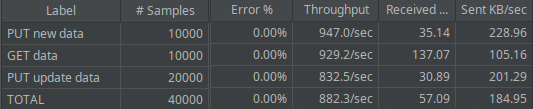
\includegraphics[width=1\textwidth]{images/stress_test_rust.png}
    \caption{Резултати тестирања \textit{Rust} сервера}
    \label{fig:stress_rust}
\end{figure}

\begin{figure}[H]
    \centering
    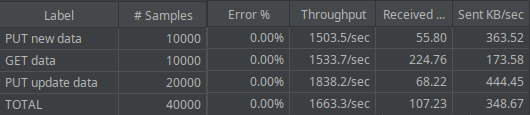
\includegraphics[width=1\textwidth]{images/stress_test_go.png}
    \caption{Резултати тестирања \textit{Go} сервера}
    \label{fig:stress_go}
\end{figure}